\documentclass[english,5p,twocolumn,preprint]{elsarticle}

\usepackage{geometry}
\geometry{margin=0.6in}

\usepackage{lineno,hyperref}
\usepackage{amsmath,amssymb,amsfonts}
\usepackage{algorithmic}
\usepackage{graphicx}
\usepackage{textcomp}
\usepackage{xcolor}
\usepackage[most]{tcolorbox}
\usepackage{listings}
\usepackage{booktabs}
\usepackage{tabularx}
\usepackage{threeparttable}
\usepackage{makecell}
\usepackage{array}
\usepackage{enumitem}

\newcommand{\EHR}{\mathrm{EHR}}
\newcommand{\KG}{\mathcal{K}}
\newcommand{\Guides}{\mathcal{G}}
\newcommand{\Dec}{\mathcal{D}}
\newcommand{\Obs}{\mathcal{O}}
\newcommand{\Risk}{\mathcal{R}}
\newcommand{\Path}{\mathcal{P}}
\newcommand{\State}{\mathcal{S}}
\newcommand{\sat}{\textsc{sat}}
\newcommand{\unsat}{\textsc{unsat}}
\newcommand{\unknown}{\textsc{unknown}}

\definecolor{codegreen}{rgb}{0,0.6,0}
\definecolor{codegray}{rgb}{0.5,0.5,0.5}
\definecolor{codepurple}{rgb}{0.58,0,0.82}
\definecolor{backcolour}{rgb}{0.95,0.95,0.92}

\lstset{
    backgroundcolor=\color{backcolour},
    commentstyle=\color{codegreen},
    keywordstyle=\color{magenta},
    numberstyle=\tiny\color{codegray},
    stringstyle=\color{codepurple},
    basicstyle=\ttfamily\small,
    breakatwhitespace=false,
    breaklines=true,
    captionpos=b,
    keepspaces=true,
    numbers=left,
    numbersep=5pt,
    showspaces=false,
    showstringspaces=false,
    showtabs=false,
    tabsize=2,
    frame=single,
    rulecolor=\color{black}
}

\modulolinenumbers[5]

\journal{Artificial Intelligence in Medicine}

\begin{document}

\begin{frontmatter}

\title{EPP: A Neuro-Symbolic Framework for the Equivalent Patient Problem in Clinical Decision Support}

\author{Mohammad Tanhaei\corref{cor1}}
\address{Department of Engineering, Ilam University, Ilam, Iran}
\ead{m.tanhaei@ilam.ac.ir}

\cortext[cor1]{Corresponding author}

\begin{abstract}
Patient similarity has become a central task in electronic health record analytics, cohort retrieval, and clinical decision support. Most existing approaches ask which patients are similar to a target patient according to raw variables, learned representations, temporal trajectories, or embedding distances. In clinical practice, however, a physician often asks a different question: which patients can be treated as equivalent for a specific decision, prognosis, or care pathway under explicit medical constraints? These two questions are not identical. Two patients may be close in an embedding space but require different therapy because of renal function, contraindications, pregnancy, drug interactions, or guideline-specific thresholds. Conversely, two patients may look dissimilar in age, body mass index, or comorbidity profile while still producing the same guideline-consistent treatment decision. 

This paper introduces the Equivalent Patient Problem (EPP) as a distinct formal problem for clinical decision support. EPP asks whether two patient states are clinically equivalent with respect to a decision space, a set of clinical guidelines, and an explicitly stated observation model. We define clinical equivalence as equality of decision-relevant outputs rather than closeness of patient descriptors. The proposed framework combines electronic health record normalization, medical knowledge graph construction, large language model assisted rule extraction, neuro-symbolic constraint construction, and satisfiability modulo theories verification. Large language models are used only as semantic-lifting components that propose candidate clinical constraints, guideline rules, and treatment preconditions, while final equivalence verdicts are issued only after symbolic validation. 

The framework distinguishes unqualified \emph{Equivalent} (which requires agreement across an approved policy set) from \emph{Equivalent under Guideline}, \emph{Non-equivalent}, \emph{Indeterminate}, and the eligibility status \emph{Out of scope}. This conservative design separates policy-relative equivalence from cases in which data are insufficient or comparison is clinically incoherent. The paper provides a formal definition, system architecture, verification conditions, illustrative diabetes, osteoporosis, and ophthalmic examples, together with an evaluation protocol. The accompanying public package provides synthetic fixtures, tests, and an audit-oriented implementation of the protocol; it does not contain patient-level BioArc data or establish clinical performance. The contribution is therefore conceptual, methodological, and software-oriented: it reframes patient similarity as decision equivalence without treating neural models as clinical oracles.
\end{abstract}

\begin{keyword}
Equivalent Patient Problem \sep Patient Similarity \sep Electronic Health Records \sep Clinical Decision Support \sep Knowledge Graphs \sep Large Language Models \sep SMT Solvers \sep Neuro-symbolic AI
\end{keyword}

\end{frontmatter}

%\linenumbers

\section{Introduction}
Electronic health records (EHRs) have enabled a broad family of data-driven clinical decision support systems. These systems use coded diagnoses, procedures, medications, laboratory tests, vital signs, and unstructured clinical notes to retrieve cohorts, predict outcomes, recommend interventions, and support observational research. A recurring primitive in these systems is patient similarity: given a target patient, retrieve patients whose records are close according to a distance metric, trajectory alignment, or learned representation \cite{allam2021patient,si2021deep,shickel2018deep}. Patient similarity is useful for cohort construction, phenotyping, risk modelling, treatment-effect estimation, and case-based reasoning.

Despite this usefulness, similarity is not the same as clinical equivalence. A distance function generally measures proximity in a representation space. Clinical decision making, in contrast, depends on thresholds, contraindications, guideline rules, institutional policies, clinician intent, patient preferences, uncertainty, and the care setting. A patient with type 2 diabetes, severe obesity, and preserved renal function may be far from another patient in demographic and comorbidity space, yet both may lead to the same medication class recommendation under a given guideline. Conversely, two patients who are nearly identical in an embedding space may diverge clinically if one has an estimated glomerular filtration rate below a contraindication threshold, a previous adverse drug reaction, pregnancy, severe hepatic disease, or an interacting medication. This distinction motivates the central sentence of this paper:

\begin{tcolorbox}[colback=gray!5,colframe=black,title=Core claim]
\centering
\textbf{Similarity is not Equivalence.}
\end{tcolorbox}

The problem is analogous to a classic distinction in program analysis. In mutation testing, two programs may look syntactically similar but differ semantically; alternatively, two programs may look different but produce the same observable output over the specified input domain. The Equivalent Mutant Problem asks whether a mutant is behaviourally equivalent to the original program under a formal observation model. This paper proposes an analogous clinical formulation: the Equivalent Patient Problem (EPP). Rather than asking whether two patient records are close, EPP asks whether two patient states produce the same decision-relevant output under explicit medical constraints.

This reframing matters because clinical decision support requires accountable outputs. A nearest-neighbour model can report that two patients are similar, but it often cannot prove that they should receive the same therapy or be assigned to the same pathway. A neural embedding may capture latent structure, but it does not by itself expose the rule that makes a clinical action valid. A guideline engine can encode rules, but it may be brittle when EHR data are incomplete, longitudinal, or expressed partly in free text.

A useful EPP framework must therefore combine representation learning, medical knowledge, guideline logic, and conservative reasoning about uncertainty. This paper introduces EPP as a formal and operational problem. The proposed framework uses EHR normalization to construct a patient state; a medical knowledge graph to represent relations among diagnoses, medications, procedures, tests, contraindications, and guideline concepts; large language models (LLMs) to extract candidate rules and preconditions from notes and guidelines; and satisfiability modulo theories (SMT) solving to verify whether two patient states are indistinguishable in the decision space. The LLM is not treated as a final clinical authority. It is used as a semantic-lifting component whose output must be typed, grounded, checked, and validated before it can affect the final verdict. This design follows a conservative neuro-symbolic principle: neural components may propose, but symbolic components must verify.

\subsection{Motivating Examples}
Consider two patients with type 2 diabetes, hypertension, and comparable glycated haemoglobin values. A standard patient-similarity model will likely place them close. If their renal function, medication history, cardiovascular risk, and contraindication profile are also comparable, they may be clinically equivalent for a first-line therapy decision. Now consider a second pair: one patient is 48 years old with body mass index 38 and no cardiovascular disease; another is 68 years old with body mass index 29 and controlled cardiovascular disease. Their raw feature vectors differ substantially. Yet, under a particular guideline and therapeutic objective, both may map to the same decision class, such as intensification with a glucose-lowering agent with cardiovascular benefit, lifestyle intervention, monitoring schedule, or referral pathway. The second pair is not necessarily similar, but it may be equivalent for a defined decision. The opposite case is also common. Two patients with similar diagnoses and laboratory values may not be equivalent if one has chronic kidney disease, a documented adverse drug reaction, pregnancy, severe frailty, or high bleeding risk. This is why EPP cannot be reduced to nearest-neighbour search. It requires a decision semantics.

\subsection{Contributions}
The paper makes four contributions.
\begin{itemize}[leftmargin=*]
    \item It defines the \emph{Equivalent Patient Problem} as a decision-centred alternative to conventional patient similarity and representation learning.
    \item It introduces a formal model of clinical equivalence in which two patient states are equivalent if they produce the same decision, prognosis category, or care pathway under explicit constraints.
    \item It proposes a neuro-symbolic architecture that combines EHR normalization, knowledge graph construction, LLM-assisted rule extraction, and SMT-based verification.
    \item It specifies conservative verdict semantics and an evaluation protocol suitable for public EHR datasets, synthetic patients, and de-identified hybrid specialty registries.
\end{itemize}

\section{Related Work}
\subsection{Patient Similarity and Representation Learning}
Patient similarity analysis aims to compare patient records across heterogeneous, longitudinal, and sparse EHR data \cite{allam2021patient}. Traditional methods use handcrafted features, distance metrics, dynamic time warping, clustering, or nearest-neighbour retrieval. Deep learning approaches instead learn patient representations directly from sequences of visits, diagnoses, medications, and laboratory events. Doctor AI used recurrent neural networks to predict future clinical events from longitudinal EHRs \cite{choi2016doctorai}. RETAIN introduced reverse-time attention to improve interpretability while preserving predictive performance \cite{choi2016retain}. BEHRT adapted transformer architectures to EHR sequences and represented disease trajectories through attention-based models \cite{li2020behrt}. Med-BERT used BERT-style pretraining on structured diagnosis records to improve prediction in low-label settings \cite{rasmy2021medbert}. 

These methods are important because they show that patient states can be represented as learned objects. However, representation learning usually optimizes predictive or retrieval objectives. It does not guarantee equality of downstream clinical decisions. Even when a representation is clinically meaningful, closeness in that representation is not equivalent to equality under a guideline, a contraindication rule, or a care pathway. EPP therefore uses representation learning as one possible source of candidate relations, not as the definition of equivalence.

\subsection{Clinical Decision Support and Guideline Formalization}
Clinical decision support systems combine patient data with medical knowledge to generate alerts, reminders, diagnostic suggestions, or treatment recommendations. Systematic reviews show that decision support can improve practice under certain design conditions, especially when integrated into workflow and delivered at the time and location of care \cite{kawamoto2005cds,sutton2020cds}. Rule-based systems have a long history in medicine, from early expert systems to modern guideline engines \cite{shortliffe1975mycin}. Guideline representation formats such as GLIF and standards such as Clinical Quality Language aim to make guideline logic executable \cite{peleg2003glif,greenes2018cql}. EPP differs from ordinary decision support. A decision support system asks: what should be recommended for this patient? EPP asks: do two patients induce the same recommendation, prognosis, or pathway under the same decision semantics? This second question is comparative and proof-oriented. It requires the system to reason about equality of outputs across patient states, not merely to compute one recommendation.

\subsection{EHR Standards, Ontologies, and Knowledge Graphs}
Clinical data are stored in heterogeneous forms. Interoperability standards and ontologies reduce this heterogeneity. OMOP CDM supports observational health research by standardizing the representation of clinical events across institutions \cite{hripcsak2015ohdsi,overhage2012omop}. HL7 FHIR defines resource-oriented data exchange for clinical systems \cite{hl7fhir2024}. SNOMED CT, LOINC, and UMLS support semantic normalization of diagnoses, observations, laboratory tests, procedures, and biomedical concepts \cite{snomed2024,loinc2024,bodenreider2004umls}. Clinical NLP systems such as cTAKES extract entities and attributes from free text \cite{savova2010ctakes}. 

A medical knowledge graph is useful for EPP because equivalence is rarely visible in raw variables. The graph can encode relations such as \emph{disease treated by medication}, \emph{drug contraindicated by renal impairment}, \emph{laboratory test measures physiological function}, \emph{procedure belongs to pathway}, or \emph{diagnosis increases risk}. These relations are the bridge between observed EHR facts and decision constraints.

\subsection{LLMs and Neuro-Symbolic Clinical Reasoning}
LLMs have demonstrated substantial clinical knowledge, but their outputs remain probabilistic and vulnerable to missing context, hallucination, and inconsistent reasoning \cite{singhal2023large,thirunavukarasu2023llm}. Recent work explores grounding LLMs in clinical practice guidelines and EHR trajectories \cite{oniani2024guidelines,li2025clicare}. This literature suggests that LLMs can assist with summarization, extraction, and guideline-aware reasoning, but it also reinforces the need for validation and auditability. EPP adopts this cautious position. The LLM is not asked to decide whether patients are equivalent. Instead, it proposes structured artefacts: candidate rules, contraindications, temporal constraints, mapping suggestions, and missing-data questions. These artefacts are translated into a typed symbolic model and checked. This differs from direct prompting, where an LLM might output an unsupported equivalence label.

\subsection{SMT Solving and Verification}
SMT solvers decide satisfiability of logical formulas modulo theories such as arithmetic, arrays, uninterpreted functions, datatypes, and bit-vectors \cite{barrett2009smt}. Z3 is a widely used SMT solver in program verification and formal reasoning \cite{moura2008z3}. In EPP, SMT is used to search for a counterexample to clinical equivalence. If the solver can find a patient-relevant condition under which two states induce different decisions, the patients are non-equivalent. If the negated equivalence condition is unsatisfiable under the model and guideline, the patients are equivalent for that model.

\section{Problem Definition}
\subsection{Patient State}
Let a patient record be represented as a tuple
\begin{equation}
    p = (X_s, X_t, N, M, L, C, F, O),
\end{equation}
where $X_s$ denotes static demographic variables (e.g., age, sex, admission time), $X_t$ denotes temporal clinical events, $N$ denotes unstructured clinical notes, $M$ denotes medications, $L$ denotes laboratory observations and vital signs, $C$ denotes coded diagnoses and comorbidities (such as multi-label ICD-11 structured selections), $F$ captures relational familial history and hereditary risks, and $O$ represents specialty-specific clinical measurements and visual examination metrics.

A normalization function maps this raw record to a typed patient state:
\begin{equation}
    \phi : \EHR \rightarrow \State.
\end{equation}
The normalized state $s=\phi(p)$ contains typed facts such as diagnosis concepts, medication exposures, laboratory values with units and timestamps, allergies, contraindications, family risk clusters, visual landmarks, and missingness indicators.

\subsection{Decision Semantics}
Let $G \in \Guides$ be a guideline or local policy, and let $\Theta_G$ be the set of medical constraints encoded from that guideline. A decision function maps a patient state to a decision vector:
\begin{equation}
    f_G : \State \times \Theta_G \rightarrow \Dec_G.
\end{equation}
The decision vector may contain medication class, dose band, monitoring interval, referral decision, diagnostic test recommendation, or pathway assignment. A prognosis function maps a patient state to a risk category or calibrated risk interval:
\begin{equation}
    r_G : \State \times \Theta_G \rightarrow \Risk_G.
\end{equation}
A pathway function maps the state to a care trajectory class:
\begin{equation}
    h_G : \State \times \Theta_G \rightarrow \Path_G.
\end{equation}
The observation model for EPP is then
\begin{equation}
    \Obs_G(s) = \left(f_G(s), r_G(s), h_G(s)\right),
\end{equation}
where individual components may be omitted depending on the application. For a medication-equivalence task, $\Obs_G$ may include only treatment class and contraindication status. For a care-pathway task, it may include referral route and monitoring schedule.

\subsection{Clinical Equivalence}
Two patient states $s_i$ and $s_j$ are clinically equivalent under guideline $G$ if they produce the same decision-relevant observation:
\begin{equation}
\label{eq:epp_guideline}
    s_i \equiv_G s_j \quad \Longleftrightarrow \quad \Obs_G(s_i) = \Obs_G(s_j).
\end{equation}
If equivalence must hold across a set of accepted guidelines or institutional policies $\Guides^*$, then global clinical equivalence is defined as
\begin{equation}
\label{eq:epp_global}
    s_i \equiv_{\Guides^*} s_j \quad \Longleftrightarrow \quad \forall G \in \Guides^*.\; \Obs_G(s_i) = \Obs_G(s_j).
\end{equation}
This definition makes the scope explicit. Equivalence is not a universal medical truth. It is always relative to a guideline set, decision space, observation model, and data completeness assumptions.

\subsection{The Equivalent Patient Problem}
Given two patient records $p_i$ and $p_j$, an observation model $\Obs_G$, and a set of constraints $\Theta_G$, the Equivalent Patient Problem asks whether
\begin{equation}
    \Obs_G(\phi(p_i)) = \Obs_G(\phi(p_j)).
\end{equation}
Equivalently, a verifier can search for a counterexample:
\begin{equation}
\label{eq:counterexample}
    \exists \theta \in \Theta_G.\; \Obs_G(\phi(p_i),\theta) \neq \Obs_G(\phi(p_j),\theta).
\end{equation}
If Eq.~\eqref{eq:counterexample} is satisfiable, the two patients are non-equivalent under $G$. If it is unsatisfiable, they are equivalent under the encoded model. If the solver returns $\unknown$, or if essential facts are missing, no equivalence claim is made. Table~\ref{tab:similarity_vs_equivalence} contrasts this model-relative task with conventional patient similarity.

\begin{table*}[ht!]
\centering
\caption{Difference between patient similarity and the Equivalent Patient Problem.}
\label{tab:similarity_vs_equivalence}
\begin{threeparttable}
\begin{tabularx}{\textwidth}{p{0.20\textwidth}p{0.35\textwidth}X}
\toprule
\textbf{Dimension} & \textbf{Patient similarity} & \textbf{Equivalent Patient Problem} \\
\midrule
Primary question & Which patients are close to this patient? & Which patients produce the same decision-relevant output under explicit clinical constraints? \\
Mathematical object & Distance, similarity score, embedding proximity, cluster membership & Equality of observations under guideline, policy, or pathway semantics \\
Typical output & Ranked list, nearest neighbours, cohort, cluster & Equivalent, Equivalent under Guideline, Non-equivalent, or Indeterminate \\
Main evidence & Feature overlap, trajectory alignment, learned representation & Constraint satisfaction, rule consistency, contraindication equality, decision equality \\
Failure mode & Similar patients may need different treatment & Equivalence may be undecidable or unsupported when data are incomplete \\
Clinical interpretability & Often indirect unless model is interpretable & Explicit because equivalence is tied to a decision rule or observation model \\
\bottomrule
\end{tabularx}
\end{threeparttable}
\end{table*}

\section{Proposed Framework}
\label{sec:framework}
The proposed framework, called EPP-NSV (Equivalent Patient Problem Neuro-Symbolic Verifier), has eight phases. The architecture follows the structure of a conservative verification system: uncertain semantic lifting is separated from proof-backed symbolic validation. Figure~\ref{fig:workflow} summarizes the evidence-bearing state, scope-gating, policy-compilation, and audit-oriented outcome flow.

\begin{figure*}[ht!]
\centering
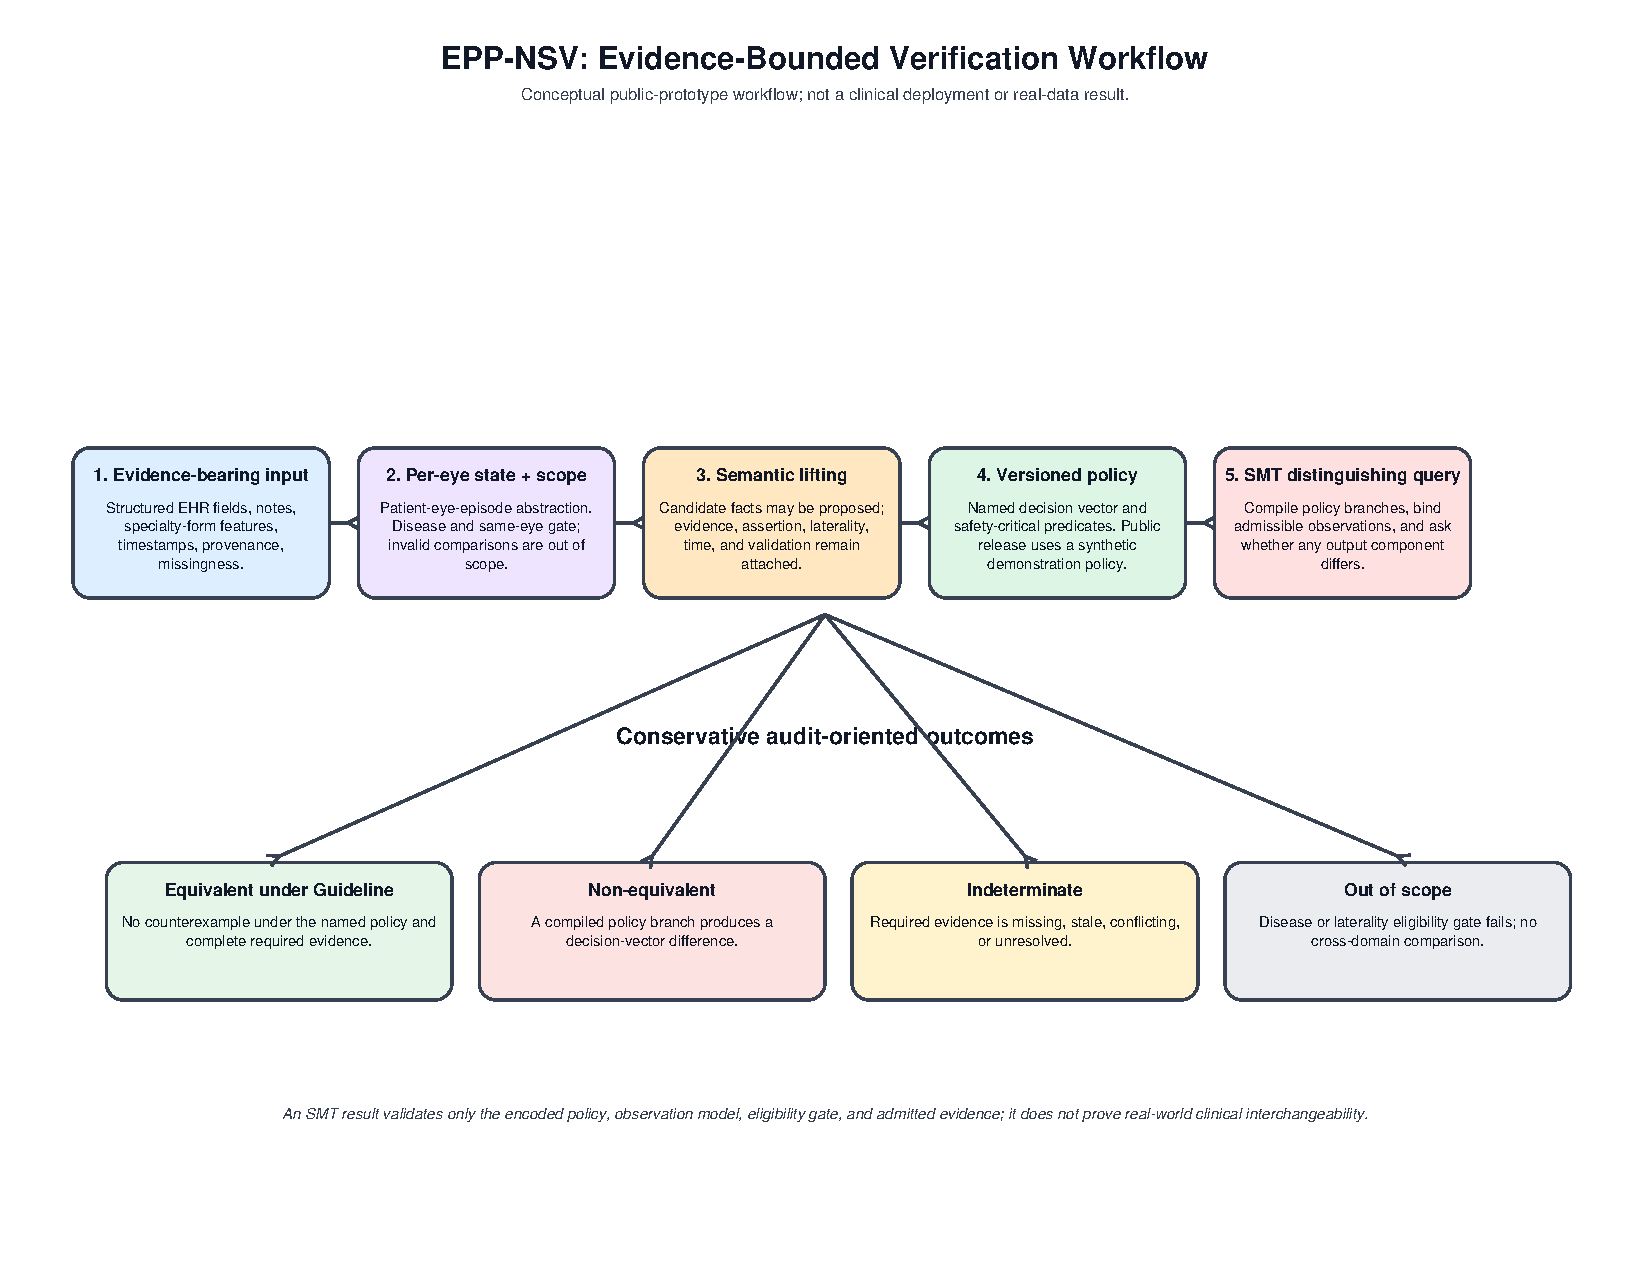
\includegraphics[width=\textwidth]{workflow.pdf}
\caption{High-level workflow of the proposed EPP-NSV framework.}
\label{fig:workflow}
\end{figure*}

\subsection{Phase 1: EHR Normalization}
The input may include diagnoses, procedures, medication orders, laboratory tests, notes, imaging reports, and longitudinal encounters. The objective of Phase 1 is not to create a single dense vector. Instead, the objective is to construct a typed state suitable for reasoning. Diagnoses are mapped to standard vocabularies, laboratory values are normalized by units and time windows, medications are mapped to active ingredients or drug classes, and note-derived facts are labelled with assertion status, temporality, and source provenance. 

For example, a raw note fragment such as ``metformin avoided because of low eGFR'' should not be stored only as free text. It should be converted to a structured assertion: \emph{metformin contraindicated or avoided}, reason: \emph{renal impairment}, source: \emph{clinical note}, timestamp: $t$, confidence: $c$. This structured form is essential because EPP depends on contraindications and treatment preconditions.

\subsection{Phase 2: Medical Knowledge Graph Construction}
The framework constructs or imports a knowledge graph $\KG=(V,E)$ where nodes represent clinical concepts and edges represent semantic relations. A simplified edge set includes:
\begin{itemize}[leftmargin=*]
    \item \texttt{disease treated\_by medication\_class},
    \item \texttt{drug contraindicated\_by condition},
    \item \texttt{lab measures physiological\_function},
    \item \texttt{condition increases risk\_of outcome},
    \item \texttt{procedure part\_of pathway},
    \item \texttt{guideline recommends action if precondition}.
\end{itemize}
The graph is not used as an opaque embedding graph. It is used to derive symbolic constraints. For instance, if the graph encodes that severe renal impairment contraindicates metformin, and the patient state encodes $eGFR < 30$, the symbolic model can derive an exclusion condition.

\subsection{Phase 3: LLM-Assisted Semantic Lifting}
LLMs can be useful for extracting guideline rules, normalizing natural language constraints, generating candidate mappings, and identifying missing information. A prompt may ask the LLM to convert a guideline paragraph into typed rules, such as:

\begin{lstlisting}[language={},caption={Illustrative rule extracted from a guideline paragraph.}]
IF patient has type_2_diabetes
AND eGFR < 30 ml/min/1.73m2
THEN metformin_status = avoid
SOURCE = guideline_G
CONFIDENCE = candidate_requires_validation
\end{lstlisting}

The key point is that this output is not accepted directly. It is parsed, mapped to the ontology, checked for type validity, compared with source text, and translated into solver constraints only after validation. If the rule cannot be grounded or conflicts with a trusted source, it is rejected or flagged for manual review.

\subsection{Phase 4: Constraint Extraction for Each Patient}
For each patient state $s$, the framework derives a constraint set $C_G(s)$ under guideline $G$. A constraint may be a Boolean fact, a numeric interval, a temporal relation, or a symbolic expression. For example:
\begin{align}
C_G(s_A) = \{& type2diabetes(s_A),\; eGFR(s_A) > 60,\\
              & no\_contraindication(s_A, metformin),\\
              & HbA1c(s_A)=8.2\}.
\end{align}
Another patient may have a different raw record but the same decision-relevant constraint abstraction:
\begin{align}
C_G(s_B) = \{& type2diabetes(s_B),\; eGFR(s_B) > 55,\\
              & no\_contraindication(s_B, metformin),\\
              & HbA1c(s_B)=7.9\}.
\end{align}
If the guideline decision only depends on diagnosis, renal threshold, contraindication status, and glycaemic threshold bands, these patients may be equivalent even though their exact values differ.

\subsection{Phase 5: Decision-Space Construction}
EPP requires an explicit decision space. Let $A_G$ be the set of candidate actions under guideline $G$. For a diabetes medication example, $A_G$ may include metformin, GLP-1 receptor agonist, SGLT2 inhibitor, insulin intensification, lifestyle intervention, monitoring-only, or specialist referral. For osteoporosis, $A_G$ may include calcium/vitamin D supplementation, bisphosphonate therapy, denosumab, anabolic therapy, fall-risk intervention, bone-density monitoring, or rheumatology referral. 

The decision function $f_G$ maps a patient state to one or more allowed actions. Equivalence can be strict or set-based. Strict decision equivalence requires the same chosen action:
\begin{equation}
    f_G(s_i) = f_G(s_j).
\end{equation}
Set-based equivalence requires the same admissible action set:
\begin{equation}
    A_G(s_i) = A_G(s_j).
\end{equation}
Set-based equivalence is often more appropriate when guidelines allow multiple clinically acceptable therapies.

\subsection{Phase 6: SMT Verification}
The symbolic bridge translates patient constraints and guideline rules into SMT formulas. The verifier checks the negation of equivalence. For set-based treatment equivalence, the counterexample formula is:
\begin{equation}
\label{eq:setcounterexample}
\begin{split}
    \exists a \in A_G.\;& \left(a \in A_G(s_i) \land a \notin A_G(s_j)\right)\\
    &\lor \left(a \in A_G(s_j) \land a \notin A_G(s_i)\right).
\end{split}
\end{equation}
If Eq.~\eqref{eq:setcounterexample} is $\unsat$, both patients have the same admissible treatment set under the model. If it is $\sat$, the model identifies an action that distinguishes the two patients. For risk equivalence, the framework can use interval equality or band equality:
\begin{equation}
    band(r_G(s_i)) = band(r_G(s_j)).
\end{equation}
For pathway equivalence, it compares pathway labels and required monitoring steps.

\subsection{Phase 7: Explanation Generation}
A clinical equivalence claim is useful only if it is explainable. The explanation module therefore returns the minimal decision-relevant facts supporting the verdict. For an equivalent pair, it may report that both patients satisfy the same diagnosis predicate, fall into the same HbA1c band, have renal function above the contraindication threshold, have no recorded drug allergy, and map to the same therapy set. For a non-equivalent pair, it reports the distinguishing condition, such as $eGFR < 30$, documented allergy, severe liver disease, high fracture risk, or missing baseline test.

\subsection{Phase 8: Missingness and Indeterminacy Handling}
EHR data are incomplete. EPP should not silently convert missing data into equivalence. If the equivalence decision depends on a missing variable, the framework reports \emph{Indeterminate} and lists the required facts. For example, if a medication recommendation depends on renal function and one patient has no recent creatinine or eGFR value, equivalence cannot be proven. This conservative treatment of missingness is central to clinical safety.

\section{Verdict Semantics}
Table~\ref{tab:verdicts} defines four decision verdicts and the separate eligibility status \emph{Out of scope}. The categories are intentionally conservative. \emph{Equivalent} is used only when the model proves equality across the selected approved policy set. \emph{Equivalent under Guideline} is used when equality holds only for a named guideline or local protocol. \emph{Non-equivalent} is used when a distinguishing decision condition is found. \emph{Indeterminate} is used when evidence is insufficient.

\begin{table*}[ht!]
\centering
\caption{Verdict semantics for EPP-NSV.}
\label{tab:verdicts}
\begin{threeparttable}
\begin{tabularx}{\textwidth}{p{0.19\textwidth}p{0.28\textwidth}X}
\toprule
\textbf{Verdict} & \textbf{Formal condition} & \textbf{Interpretation} \\
\midrule
Equivalent & $\Obs_G(s_i)=\Obs_G(s_j)$ and the negated condition is $\unsat$ under the selected model & The two patients are decision-equivalent for the stated observation model, guideline set, and data assumptions. \\
Equivalent under Guideline $G$ & $\Obs_G(s_i)=\Obs_G(s_j)$, but equivalence is not proven across all guideline variants or institutional policies & The two patients are equivalent only under the named guideline, protocol, or local policy. \\
Non-equivalent & The solver finds a satisfying assignment for $\Obs_G(s_i)\neq\Obs_G(s_j)$ & A decision-relevant difference exists; the explanation should identify the differentiating rule or clinical fact. \\
Indeterminate & Translation fails, solver returns $\unknown$, a required fact is missing, or the model omits a relevant clinical effect & No equivalence claim is made; additional data, manual review, or a stronger model is required. \\
Out of scope & Disease, laterality, or task-eligibility gate fails before decision comparison & No clinical-equivalence statement is attempted because the comparison is not meaningful under the stated task definition. \\
\bottomrule
\end{tabularx}
\end{threeparttable}
\end{table*}

\section{Illustrative Case Studies}
\subsection{Diabetes Medication Equivalence}
Assume a simplified diabetes guideline with three rules: metformin is admissible for type 2 diabetes when renal function is above a threshold and no contraindication is recorded; an SGLT2 inhibitor is preferred when cardiovascular or renal benefit is indicated and not contraindicated; insulin intensification is considered when glycaemic control exceeds a specified band despite therapy. Let patient $A$ be 55 years old with diabetes, hypertension, HbA1c 8.2, and eGFR 70. Let patient $B$ be 61 years old with diabetes, hypertension, HbA1c 7.9, and eGFR 65. A similarity system may retrieve $B$ because the raw features are close. EPP asks whether the same medication set is admissible.

If both patients fall into the same HbA1c decision band and have no contraindication, the solver may prove:
\begin{equation}
    A_G(s_A) = A_G(s_B).
\end{equation}
The verdict is \emph{Equivalent} for the specified medication decision. The explanation should not say that the patients are medically identical. It should say that the encoded decision function cannot distinguish them for the selected therapy decision.

Now consider patient $C$ with eGFR 25 and patient $D$ with eGFR 65. The similarity score may still be high if the model gives renal function low weight. EPP will classify the pair as \emph{Non-equivalent} if the metformin rule distinguishes them. The counterexample is the renal threshold condition.

\subsection{Obesity, Cardiovascular Disease, and Same Treatment Pathway}
Consider two patients with type 2 diabetes. Patient $E$ is younger with severe obesity and no documented cardiovascular disease. Patient $F$ is older with lower body mass index and controlled cardiovascular disease. Their raw demographics and comorbidity profiles differ. However, if the guideline maps both to the same admissible treatment set because both require intensification and both have no contraindication to a target drug class, EPP may report equivalence under that guideline. This case illustrates why equivalence is not feature proximity. The feature vectors are different, but the decision-relevant abstraction is the same. A useful clinical decision support system should be able to make this distinction explicit.

\subsection{Osteoporosis Registry Example}
An osteoporosis registry can provide another natural domain. Treatment decisions may depend on age band, history of fragility fracture, bone mineral density, glucocorticoid exposure, renal function, calcium level, dental risk, previous bisphosphonate exposure, and fracture-risk category. Two patients may have different detailed histories but the same treatment pathway: antiresorptive therapy, supplementation, fall-risk assessment, and follow-up dual-energy X-ray absorptiometry interval. EPP can formalize whether their pathway assignment is equal under a selected osteoporosis guideline. This example also shows the value of registry data. A registry usually contains curated disease-specific variables that are closer to the decision space than raw EHR data. However, the EPP verifier should still represent missingness, contraindications, and guideline versioning because equivalence can change when a guideline changes.

\subsection{Ophthalmology and Hybrid EHR Registries: The BioArc Ecosystem}
Unlike general-purpose generic EHR datasets, domain-specific health data ecosystems provide a structured clinical form that naturally decomposes the patient state into decision-relevant components. This enables a precise formal definition of patient equivalence within a highly constrained clinical decision space, precluding the clinical invalidity of comparing unrelated clinical domains (e.g., matching an ophthalmic patient against a cardiac baseline). 

Consider an ophthalmology registry built on a hybrid architecture, where the patient state encompasses multiple distinct architectural layers:
\begin{equation}
    S_{patient} = \{D, C_{ICD}, H_F, H_C, M_O, T\},
\end{equation}
where $D$ represents explicit demographics (age, sex, and precise admission data), $C_{ICD}$ is a structured ICD-11 disease state mapping primary diagnoses and multi-label comorbidities into a unified ontology layer, $H_F$ captures relational familial history and hereditary risk distributions, $H_C$ contains unstructured clinical history and free-text physician notes extractable via semantic LLM lifting, $M_O$ holds specialty-specific ophthalmic examinations, and $T$ represents the fine-grained temporal ordering layer.

In this architecture, defining the Equivalent Patient Problem transforms into a constrained verification task:
\begin{equation}
    EPP(p_i, p_j) \iff \Obs_G(S_i) = \Obs_G(S_j) \text{ under } \Theta_{eye},
\end{equation}
where the constraint set $\Theta_{eye}$ explicitly evaluates visual thresholds, structural degradation, and hereditary risk modifiers against guideline-based rules. Two patients may present with entirely different text-based chief complaints; however, if their structured $C_{ICD}$ layer and $M_O$ parameters satisfy identical threshold constraints under $\Theta_{eye}$, the neuro-symbolic verifier mathematically proves them to be \emph{Equivalent} within that decision boundary.

\subsubsection{Visual-to-Symbolic State Abstraction in Specialty Registries}
In advanced specialty registries, clinical observations are frequently captured via interactive visual modules (e.g., click-based anatomical landmarks) rather than raw free text. Translating these spatial and visual annotations into a structured feature space is a critical realization of the neuro-symbolic semantic lifting described in Phase 3 of EPP-NSV.

When visual data is directly mapped to a constrained state space, the solver can seamlessly verify clinical equivalence. Table~\ref{tab:visual_abstraction} illustrates how specific interactive ophthalmic modules are translated into symbolic state variables and directly influence the decision output space.

\begin{table*}[ht!]
\centering
\caption{Mapping interactive ophthalmic examination modules to EPP state variables and corresponding decision spaces.}
\label{tab:visual_abstraction}
\begin{tabularx}{\textwidth}{p{0.20\textwidth}p{0.45\textwidth}X}
\toprule
\textbf{Clinical Module} & \textbf{Symbolic State Space ($\State$)} & \textbf{Target Decision Output Space ($\Dec_G$)} \\
\midrule
\textbf{Anterior Segment \& Angle} & \texttt{angle\_status} $\in \{open, occludable\}$, \texttt{chamber\_depth} $\in \{shallow, deep\}$, \texttt{lens\_opacity\_severity} & Glaucoma surgical intervention, Cataract surgery indication \\
\addlinespace
\textbf{Fundus Examination} & \texttt{cupping\_ratio} $\in [0,1]$, \texttt{macula\_edema} $\in \{true, false\}$, \texttt{retinal\_tears} & Anti-VEGF medical therapy, Vitreoretinal surgery pathway \\
\addlinespace
\textbf{Strabismus Module} & \texttt{angle\_of\_deviation} (degrees), \texttt{fixation\_pattern}, \texttt{binocular\_function} & Strabismus surgical planning, Amblyopia management \\
\addlinespace
\textbf{External Eye Exam} & \texttt{eyelid\_position} $\in \{normal, ptosis\}$, \texttt{corneal\_surface\_clarity} & Oculoplastic referral, Corneal disease management \\
\bottomrule
\end{tabularx}
\end{table*}

This explicit mapping transforms subjective visual assessments into formal constraints. For instance, two patients may differ significantly in their raw Fundus images; however, if their extracted state vectors both satisfy the condition $macula\_edema = true$ and share the same structured treatment decision within the Treatment Panel output space (e.g., $Vitrectomy$ or $Anti-VEGF$), they are mathematically proven to be \emph{Equivalent} within the defined surgical decision space.

\section{Implementation Design}
\subsection{Data Model}
The implementation can use OMOP CDM or FHIR as an interoperability layer. OMOP is useful for observational research and cohort-level analysis, while FHIR is useful for resource-based exchange with clinical systems. The EPP internal representation should be independent of either standard. A practical implementation can define adapters:
\begin{equation}
    adapter_{OMOP}: OMOP \rightarrow \State,
\end{equation}
\begin{equation}
    adapter_{FHIR}: FHIR \rightarrow \State.
\end{equation}
This separation allows EPP to be tested on public datasets such as MIMIC-IV, eICU, and Synthea, and then deployed on institutional registries after de-identification and governance approval \cite{johnson2023mimiciv,pollard2018eicu,walonoski2018synthea}.

\subsection{Rule Schema}
Every rule is represented using a typed schema:
\begin{equation}
\begin{split}
    rule = (&preconditions, action, exceptions,\\
            &source, version, confidence).
\end{split}
\end{equation}
Preconditions are logical formulas over patient facts. Exceptions represent contraindications or exclusion criteria. Source and version are required because guideline rules change. Confidence is not used to prove equivalence; it is used only to prioritize review. A low-confidence rule cannot support an \emph{Equivalent} verdict unless it is manually accepted or validated against a trusted source.

\subsection{Solver Encoding}
The solver encoding uses Boolean predicates for categorical facts, linear arithmetic for numeric thresholds, finite enumerations for medication classes, and uninterpreted functions when detailed pharmacological mechanisms are outside the model. For example:
\begin{lstlisting}[language={},caption={Simplified SMT-style representation.}]
(declare-const has_T2D_A Bool)
(declare-const has_T2D_B Bool)
(declare-const eGFR_A Real)
(declare-const eGFR_B Real)
(declare-const metformin_allowed_A Bool)
(declare-const metformin_allowed_B Bool)
(assert (= metformin_allowed_A
           (and has_T2D_A (>= eGFR_A 30))))
(assert (= metformin_allowed_B
           (and has_T2D_B (>= eGFR_B 30))))
(assert (not (= metformin_allowed_A metformin_allowed_B)))
(check-sat)
\end{lstlisting}
If the final assertion is unsatisfiable under patient constraints, the patients are equivalent for the metformin-admissibility decision. If satisfiable, the model reveals the distinguishing condition.

\subsection{Audit Log}
Every verdict should be accompanied by an audit log containing the patient-state extraction version, vocabulary mappings, guideline sources, LLM prompts and outputs, accepted rules, rejected rules, solver formulas, solver version, and final model or proof status. This is essential for reproducibility and clinical governance. It also prevents the system from becoming a black-box similarity engine.


\section{Experimental Evaluation Protocol}
This paper does not fabricate empirical results. Instead, it specifies an evaluation protocol that can be executed once de-identified data and clinical adjudication are available. The protocol is designed to answer five research questions.

\subsection{Research Questions}
\begin{itemize}[leftmargin=*]
    \item \textbf{RQ1:} How often do similarity and equivalence disagree?
    \item \textbf{RQ2:} Does EPP-NSV identify clinically equivalent pairs that embedding-based similarity models rank as distant?
    \item \textbf{RQ3:} Does EPP-NSV identify non-equivalent pairs that similarity models rank as close?
    \item \textbf{RQ4:} What fraction of cases become \emph{Indeterminate} because of missing data, unsupported rules, or solver limitations?
    \item \textbf{RQ5:} How sensitive are verdicts to guideline version, rule source, and observation model?
\end{itemize}

\subsection{Datasets}
Table~\ref{tab:datasets} lists candidate datasets. Public datasets allow reproducibility, synthetic datasets allow safety testing, and de-identified registries allow disease-specific validation.

\begin{table*}[ht!]
\centering
\caption{Candidate data sources for evaluating EPP.}
\label{tab:datasets}
\begin{tabularx}{\textwidth}{p{0.20\textwidth}p{0.23\textwidth}X}
\toprule
\textbf{Dataset type} & \textbf{Example} & \textbf{Role in evaluation} \\
\midrule
Public critical-care EHR & MIMIC-IV, eICU & Reproducible testing of extraction, missingness handling, and guideline-local equivalence in selected decision tasks. \\
Synthetic EHR & Synthea & Controlled generation of patient pairs with known decision differences and privacy-safe stress testing. \\
Disease registry & Osteoporosis registry & Disease-specific equivalence tasks with curated variables and expert adjudication. \\
Hybrid Specialty Registry & BioArc Ophthalmology Ecosystem & Evaluates EPP on a multi-layered state space combining structured ICD-11 codes, free-text clinical notes, relational familial history, and specialty visual/interactive modules. \\
Institutional EHR & De-identified private EHR & Real-world validation across local workflows, coding practices, and clinical policies. \\
Guideline corpus & Public guideline text & Source material for rule extraction, versioning, and guideline-specific equivalence. \\
\bottomrule
\end{tabularx}
\end{table*}

\subsection{Pair Construction}
Evaluation requires labelled patient pairs. Pairs can be constructed in four ways. First, nearest-neighbour pairs are selected using conventional patient similarity models. These test whether similarity implies equivalence. Second, distant pairs are selected from different embedding regions. These test whether raw dissimilarity can hide decision equivalence. Third, synthetic counterfactual pairs are generated by changing one clinically relevant variable, such as renal function or allergy status. These test whether the verifier detects non-equivalence. Fourth, expert-selected pairs are provided by clinicians from registry review.

\subsection{Baselines}
A complete evaluation should compare EPP-NSV with several baselines:
\begin{itemize}[leftmargin=*]
    \item nearest-neighbour retrieval over handcrafted EHR features;
    \item dynamic time warping or trajectory similarity for longitudinal events;
    \item patient embeddings from recurrent or transformer models;
    \item contrastive patient-representation learning;
    \item direct LLM judgement without symbolic verification;
    \item rule-only guideline execution without LLM-assisted extraction.
\end{itemize}
The direct LLM baseline is important because it tests whether neuro-symbolic verification adds value beyond prompting. The expectation is not that EPP-NSV will label every pair; rather, it should avoid unsupported equivalence claims.

\subsection{Metrics}
The primary metrics are precision and recall for \emph{Equivalent} and \emph{Non-equivalent} labels against expert adjudication. However, EPP also requires metrics for abstention and explanation:
\begin{itemize}[leftmargin=*]
    \item \textbf{Equivalence precision:} fraction of \emph{Equivalent} verdicts accepted by clinicians.
    \item \textbf{Non-equivalence precision:} fraction of distinguishing conditions accepted by clinicians.
    \item \textbf{Indeterminate rate:} fraction of pairs for which no safe verdict is issued.
    \item \textbf{Explanation adequacy:} clinician rating of whether the decisive facts are visible and correct.
    \item \textbf{Guideline sensitivity:} fraction of verdicts that change across guideline versions.
    \item \textbf{Similarity-equivalence disagreement:} fraction of pairs where embedding distance and EPP verdict conflict.
\end{itemize}

\subsection{Ablation Study}
An ablation study should remove one component at a time: the knowledge graph, LLM-assisted extraction, symbolic verification, missingness logic, and guideline versioning. The key hypothesis is that removing symbolic verification will increase unsupported equivalence claims, while removing LLM-assisted extraction will reduce coverage because fewer rules and constraints are available.

\section{Discussion}
\subsection{Why EPP is Not Just Better Similarity}
One might argue that EPP can be solved by learning a better representation. A representation could be trained so that clinically equivalent patients are close. This is useful, but it does not eliminate the need for EPP. First, equivalence is task-dependent. Two patients may be equivalent for one medication decision but not for surgical risk, follow-up frequency, or prognosis. Second, equivalence is guideline-dependent. A new contraindication or threshold can change the decision boundary. Third, equivalence needs explanations because clinicians need to know why two patients are treated alike. Fourth, missing data must produce abstention rather than artificial closeness. A learned representation can therefore support EPP by proposing candidate pairs or by learning soft similarity within a decision space. It should not define equivalence on its own. EPP requires an explicit observation model and a checkable decision semantics.

\subsection{Clinical Safety and Governance}
EPP should not be used as an autonomous treatment system. It is a decision-support and research framework for comparing patient states under explicit assumptions. Clinical deployment requires governance, validation, local guideline review, monitoring for bias, and clear human oversight. The safest use cases are retrospective cohort review, registry analysis, decision-support audit, and clinician-facing explanation of why a system grouped patients together. The framework also exposes a governance benefit. If a system reports that two patients are equivalent, it must state the guideline, decision space, relevant facts, missing variables, and solver result. This is more auditable than a similarity score alone.

\subsection{Relationship to Personalized Medicine}
At first glance, equivalence may appear to conflict with personalized medicine. Personalized medicine emphasizes individual differences, whereas equivalence groups patients. The apparent conflict disappears once equivalence is defined relative to a decision. EPP does not claim that two patients are identical. It claims that no decision-relevant difference is visible under the current model. This can actually support personalization by identifying which differences matter and which differences do not matter for a specific decision.

\subsection{Potential Extensions}
Future versions can extend EPP beyond deterministic guideline rules. Probabilistic EPP can define equivalence over calibrated risk intervals. Causal EPP can define equivalence over expected treatment effect rather than outcome risk alone. Temporal EPP can compare full care trajectories over time. Multi-guideline EPP can quantify when equivalence is robust across institutions or fragile under guideline changes. Federated EPP can support cross-site verification without moving patient-level data.

\section{Limitations and Threats to Validity}
\subsection{Conceptual Scope}
EPP is a new problem formulation, not a claim that all clinical decisions can be reduced to symbolic rules. Many decisions depend on patient preference, clinician judgement, resource availability, local constraints, and uncertainty that may not be fully encoded. The proposed framework applies only to the decision space that is explicitly modelled.

\subsection{Data Quality}
EHR data are incomplete, noisy, and biased. Missing laboratory values, outdated medication lists, inconsistent coding, and unstructured notes can affect equivalence. The framework mitigates this risk by reporting \emph{Indeterminate} when required facts are missing. This protects precision but may reduce coverage.

\subsection{Guideline Variability}
Guidelines evolve and may conflict. A pair can be equivalent under one guideline and non-equivalent under another. This is not a defect; it is part of the problem definition. The framework must therefore record guideline source and version.

\subsection{LLM Reliability}
LLMs can extract useful candidate rules, but they can hallucinate, omit exceptions, or overgeneralize. EPP-NSV mitigates this by treating LLM output as a hypothesis. A candidate rule must be grounded, typed, validated, and auditable before use. When validation fails, the system abstains or requests manual review.

\subsection{Solver Limitations}
SMT solving is powerful but not complete for all clinical modelling problems. Nonlinear risk models, probabilistic dependencies, temporal uncertainty, and free-text ambiguity may exceed the solver's tractable fragment. The correct response is not to force a label; it is to report \emph{Indeterminate} or use a bounded/verifiable approximation. Table~\ref{tab:limitations} summarizes the principal threats and intended mitigations.

\begin{table*}[ht!]
\centering
\caption{Major limitations and mitigations.}
\label{tab:limitations}
\begin{tabularx}{\textwidth}{p{0.24\textwidth}p{0.30\textwidth}X}
\toprule
\textbf{Limitation} & \textbf{Consequence} & \textbf{Mitigation} \\
\midrule
Incomplete EHR data & False equivalence if missing values are ignored & Explicit missingness logic and \emph{Indeterminate} verdict. \\
Guideline ambiguity & Different sources may produce different verdicts & Guideline-specific equivalence and versioned rule provenance. \\
LLM hallucination & Incorrect candidate rules & Grounding, type checking, source comparison, and symbolic validation. \\
Unsupported clinical concepts & Loss of coverage & Extend ontology mappings and report unsupported cases. \\
Solver unknown results & No proof or counterexample & Split formulas, simplify models, or abstain. \\
Clinician judgement not encoded & Model may omit contextual factors & Human review and explicit observation-model boundaries. \\
\bottomrule
\end{tabularx}
\end{table*}

\section{Conclusion and Future Work}
This paper introduced the Equivalent Patient Problem as a distinct decision-centred formulation for clinical decision support. Existing patient similarity systems ask which patients are close in feature, trajectory, or embedding space. EPP asks which patients are equivalent with respect to a treatment decision, prognosis category, or care pathway under explicit clinical constraints. The distinction is important because two similar patients may require different actions, while two dissimilar patients may map to the same guideline-consistent decision. 

The proposed EPP-NSV framework combines EHR normalization, medical knowledge graphs, LLM-assisted semantic lifting, typed symbolic modelling, and SMT verification. The main design principle is conservative neuro-symbolic reasoning: LLMs generate candidate artefacts, but equivalence verdicts require symbolic validation. The framework reports four outcomes: \emph{Equivalent}, \emph{Equivalent under Guideline}, \emph{Non-equivalent}, and \emph{Indeterminate}. This verdict design makes the scope of every claim explicit and avoids treating missing information as proof. 

Future work should implement the framework on a public benchmark, create expert-adjudicated patient-pair labels, test disease-specific hybrid registries such as the BioArc ophthalmology ecosystem, and evaluate how often similarity and equivalence disagree. Another important direction is privacy-preserving deployment, where local EHR systems compute patient states and verification artefacts without exporting identifiable records. Finally, probabilistic and causal extensions should define equivalence not only over guideline actions but also over expected treatment effects and uncertainty-calibrated prognosis.

\section*{Code and Data Availability}
The EPP-NSV source code, synthetic fixtures, unit tests, and controlled-study documentation are available at \url{https://github.com/tanhaei/EPP} \cite{tanhaei2026epp}. The public repository contains no BioArc patient-level data, real clinical-note corpus, or real-data result bundle. This manuscript is a methodological and protocol-scope paper; the public experiments validate software behavior on constructed fixtures only. Any future empirical study must use de-identified data under the applicable institutional approval, data-use agreement, and governance process. Access to controlled BioArc data, if approved, must proceed through the platform's authorized research-access pathway and cannot be inferred from this public release.

\section*{Clinical Safety Statement}
The framework proposed in this paper is intended for research, audit, and clinician-supervised decision support. It is not a substitute for professional medical judgement and must not be used as an autonomous treatment system.

\bibliographystyle{elsarticle-num}
\bibliography{bibliography}

\end{document}
